\section{Envisioned final product}
A lot to be critical about this design, e.g. it doesn't really account for how braille is read and the convenience of keeping one's fingers in place. It is essentially a braille version of a sighted product.
\begin{figure}[h]
\centering
    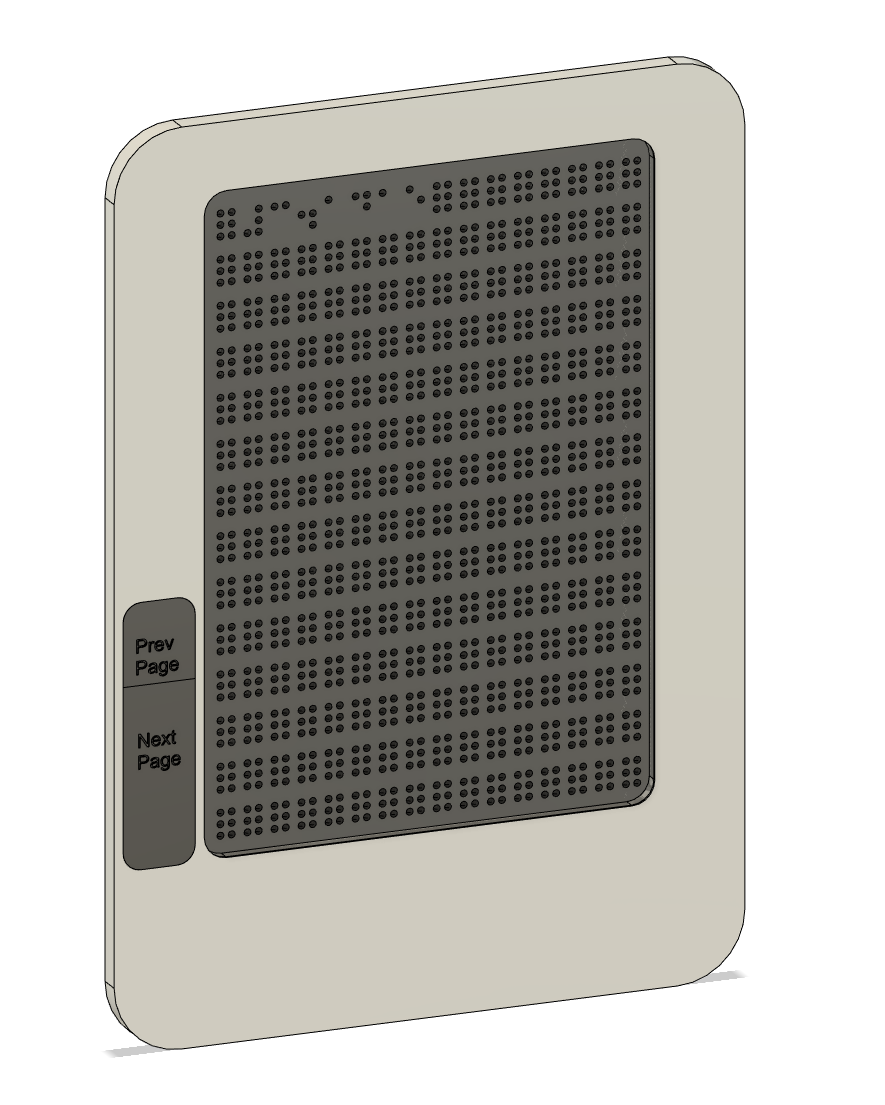
\includegraphics[width=0.4\textwidth]{figures/e-reader.png}
\caption[Envisioned finished product]{Envisioned finished product. A Braille version of a standard e-reader aimed to provide broadened access and display information a traditional Braille device can't.}
\label{fig:e-reader.png}
\end{figure}

% \subsection{Encoding}
% Figure \ref{fig:encoding.png} describes the initial approach to convert text into braille given a device with 16 addressable cells.
% \begin{figure}[h]
% \centering
%     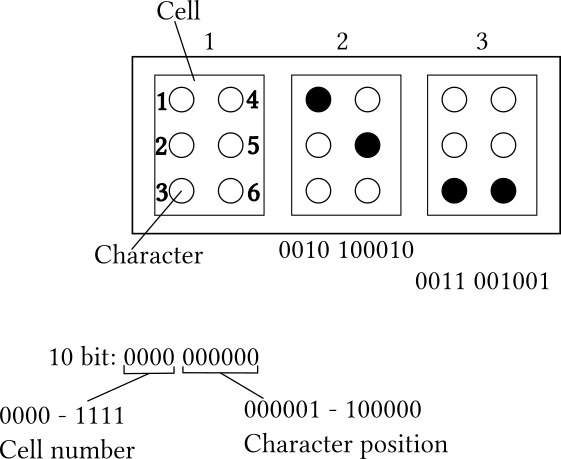
\includegraphics[height=5cm]{figures/encoding.png}
% \caption{Early idea for serial encoding of up to 16 braille cells.}
% \label{fig:encoding.png}
% \end{figure}

\section{Actuator technology}
    \subsection{Addressable cell}
    Use of a typing element similar to IBM Selectric typewriter as shown in figure \ref{fig:IBM_Selectric_Globe_Wiki.jpg}. Viable for a printer, however the moving mechanism is too large to be embedded into a tablet-sized device. Hybrid addressable cell attempts to tackle the size issue.
    \begin{figure}[h]
    \centering
        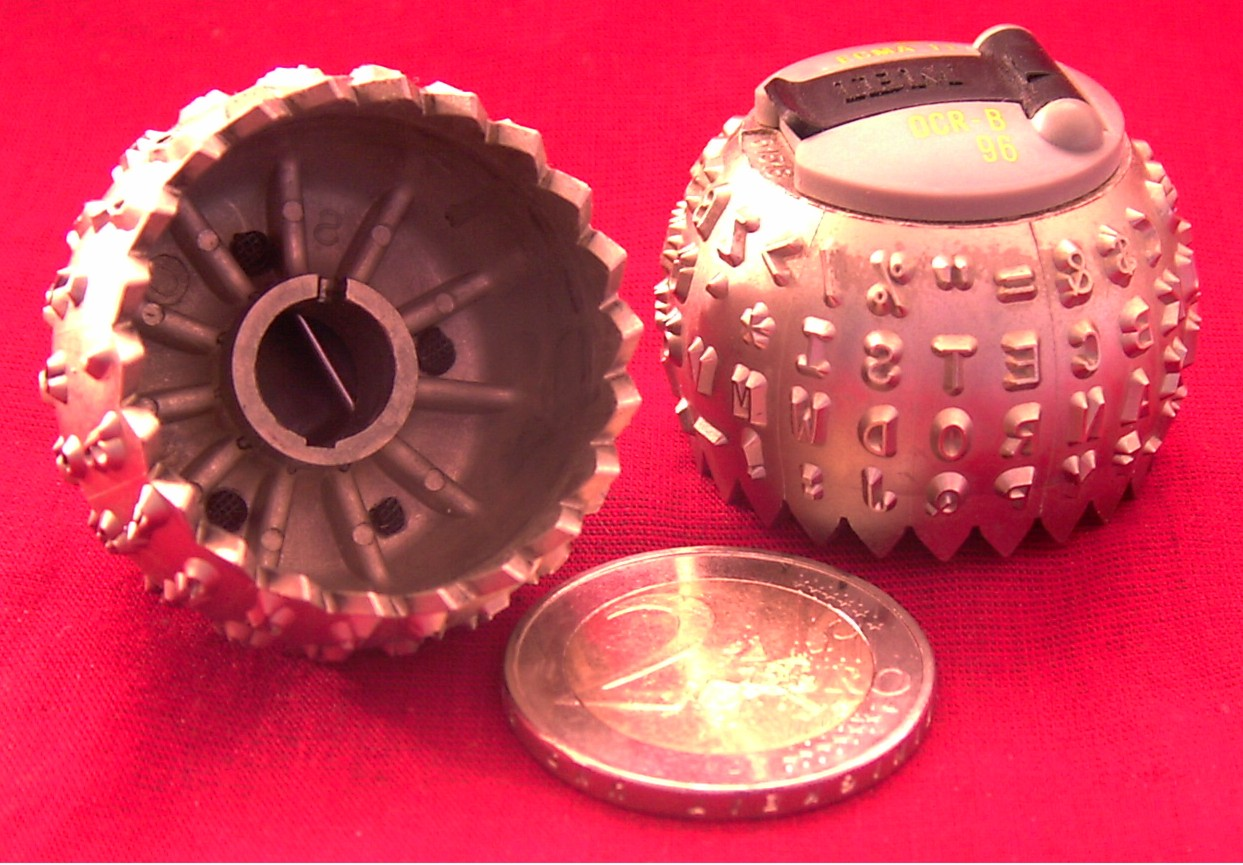
\includegraphics[height=5cm]{figures/IBM_Selectric_Globe_Wiki.jpg}
    \caption[IBM Selectric typing element]{IBM Selectric typing element \cite{wiki:IBMSelectric}.}
    \label{fig:IBM_Selectric_Globe_Wiki.jpg}
    \end{figure}

    An alternative that addresses the size is shown in figure \ref{fig:rotation.png}, wherein the characters fall partially into a slot, resulting in their depression on the surface. Each rotating disk is a saggital half of the braille cell, i.e. two disks form one braille cell. Roberts et al explore similar ideas \cite{roberts_492_2000}, and faced issues with component wear and the mechanism jamming.

    \begin{figure}[h]
    \centering
        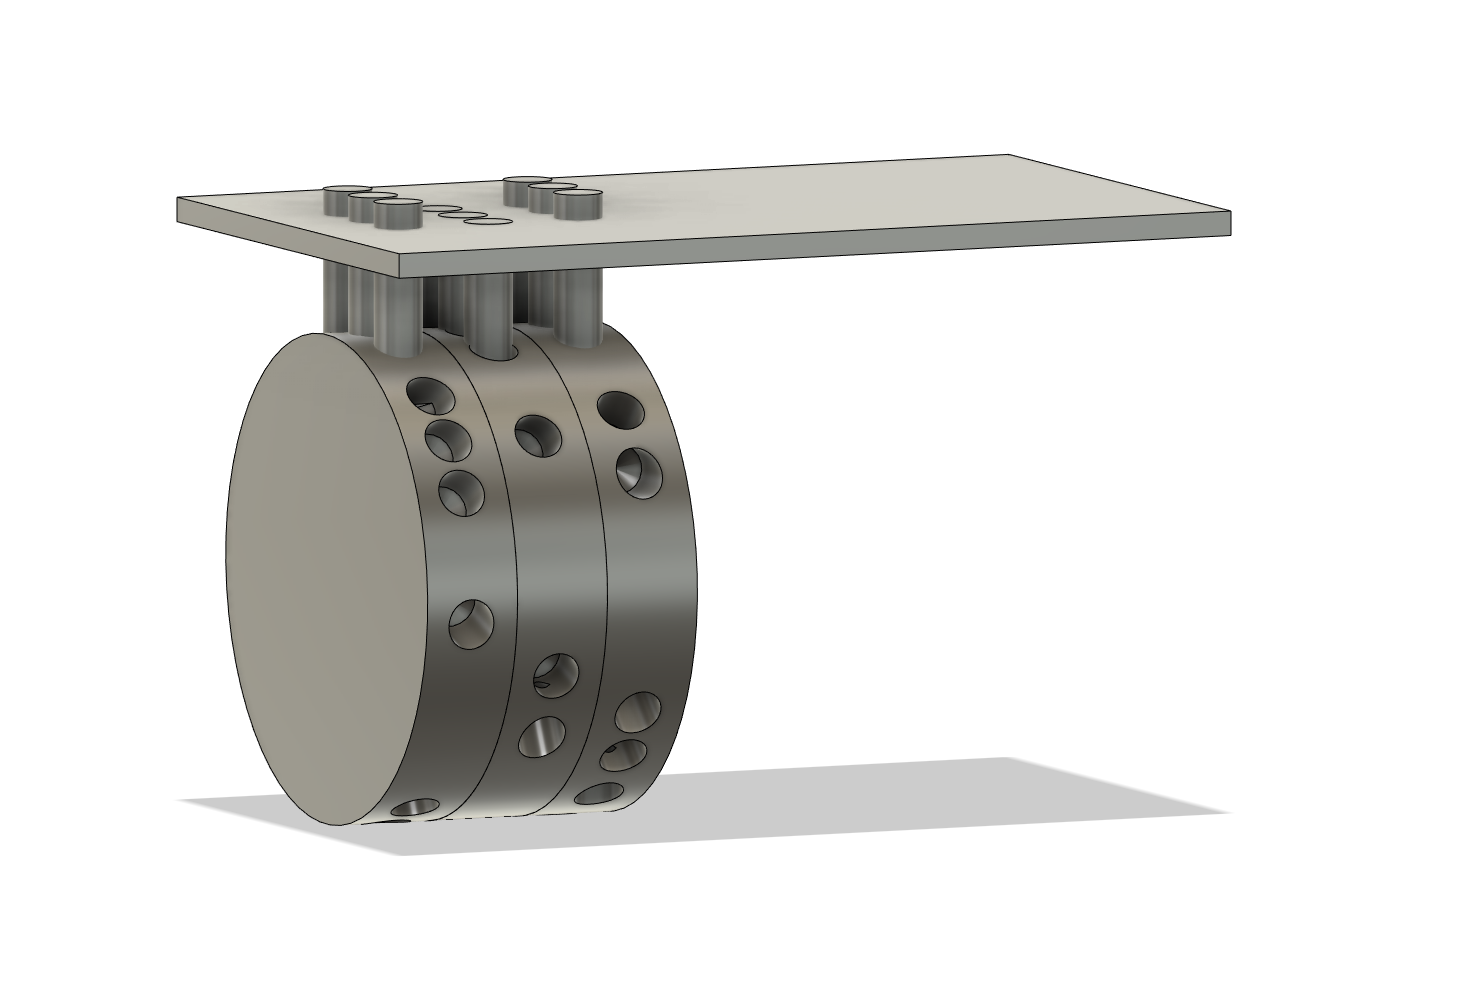
\includegraphics[width=0.6\textwidth]{figures/rotation.png}
    \caption{Hybrid addressable cell. Holes on the disk define which pins are depressed on the surface.}
    \label{fig:rotation.png}
    \end{figure}

    \subsection{Individually addressable characters}
    \subsubsection{Electromechanical}
    This includes piezoelectric and the linear actuators. Not considered due to size. Examples will be addressed in the status quo analysis.

    \subsubsection{Pneumatic}
    Usage similar to \cite{XieZhixin2021A2rB}. Use of a compliant mechanism for a bi-stable switch of the character.  
    \begin{figure}[h]
    \centering
        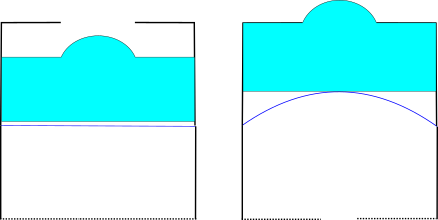
\includegraphics[height=5cm]{figures/pneumatic.png}
    \caption{Pneumatic actuation mechanism}
    \label{fig:pneumatic.png}
    \end{figure}

    \subsubsection{Magnetic}
    \paragraph{Linear actuators} % Both latch and standard linear we're doing

    \paragraph{Ferromagnetic fluids}
    Despite its early developmental stage, the use of ferromagnetic fluids is promising \cite{fletcher_magnetic_2021}.
    Character in a cell are individually created by their correspondent electromagnet, and can reasonably meet the UK Association for Accessible Formats (UKAAF) standards.
    Given it is at a proof-of-concept stage, producing it for this study is unreasonable.
    \paragraph{Others} % Magnet on rail
    Generally the technologies used for actuation push the pin out of a socket.
    The research of \cite{loconsole_braillecursor_2019} explores the use of passive pins and a magnetic rail that pulls each pin, then drops them in a given position that results in up or down. Figure \ref{fig:magnetic-rail} shows this scheme.
    While the reduced energy consumption due to passive components is appealing, this solution has an error rate of at least 5\%, and each row of cells necessitates a large motor.
    \begin{figure}[h]
    \centering
        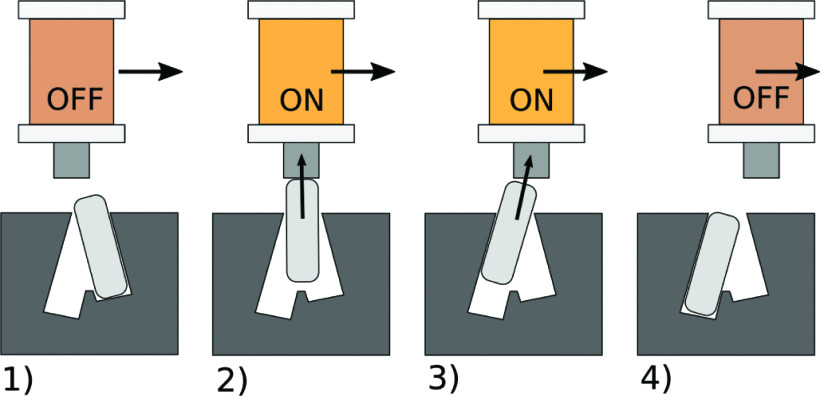
\includegraphics[width=0.6\textwidth]{figures/magnetic-rail.jpg}
    \caption{Magnetic rail actuation mechanism. Pins are magnetically pulled from the socket and deposited in either position, having them be on or off (or up and down)}
    \label{fig:magnetic-rail}
    \end{figure}  

    Linear motion electromagnetic actuator as seen in figure \ref{fig:magnet-cross_section.png}.
    It consists of a variable magnet at the base that pushes a permanent magnet attached to the character. Its largest problem is size, which is briefly discussed by \cite{BettelaniGemmaCarolina2020DaVo}.


    Overcoming the need for a continuous magnetic field that pushes a character up has been partially solved by the usage of a latch \cite{KimJoonyeong2020BDfP}. Results are questionable, and we end up with a design that is very similar to the pneumatic with a compliant mechanism.


    \begin{figure}[h]
    \centering
        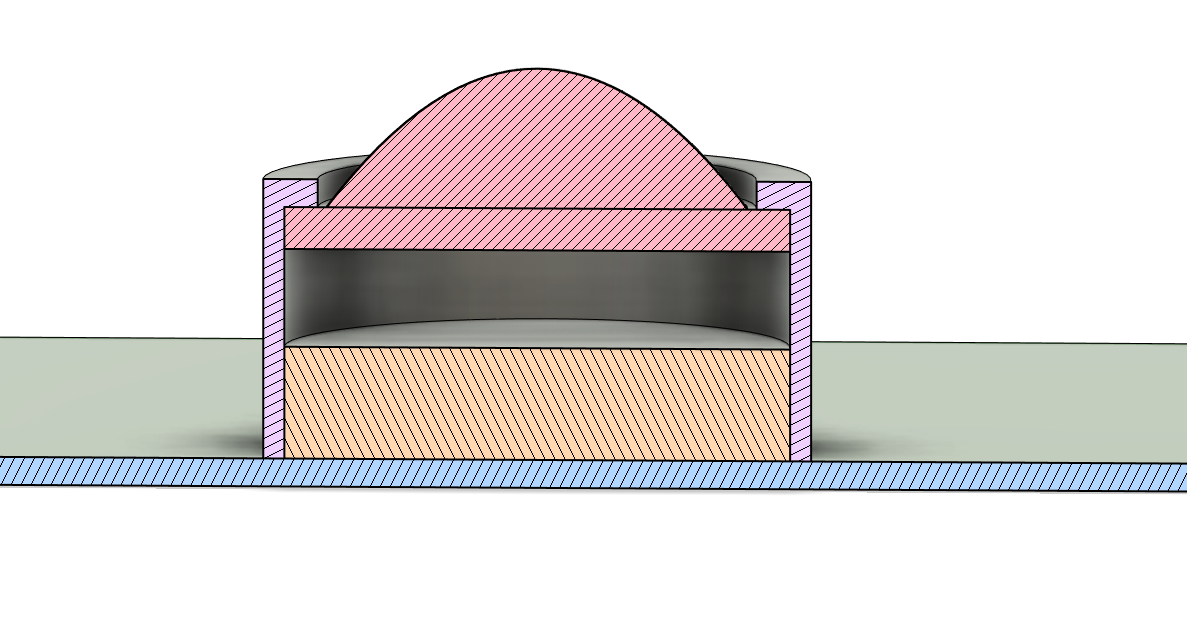
\includegraphics[height=5cm]{figures/magnet-cross_section.png}
    \caption{Cross-section of magnetic actuator}
    \label{fig:magnet-cross_section.png}
    \end{figure}


